\section{Implementation}

\subsection{Platform}
\begin{figure}
\includegraphics[keepaspectratio, width=0.35\textheight]
{../presentation/img/architecture-diagram.png}
\caption{Architecture of our current platform. Clients are aware of the partition that
holds the initial vertex of a query. The server that accepted the request becomes the
coordinator, communicates with other servers, and replies to the client with a full
answer}
\label{fig:architecture}
\end{figure}

Our implementation of the graph database system can be seen on Figure
\ref{fig:architecture}. Our current platform implements hash partitioning due 
to its simplicity. All components have to include the partition manager in order
to know where to submit the requests. One major advantage of this scheme is that
clients will see reduced latencies, because they can communicate directly to the
partition that is holding a vertex.

Each server uses MySQL as a stand-alone database instance (each instance is
unaware of other instances). Every time a server accepts a request from a client,
it becomes the coordinator for that query and will likely communicate with
other servers in order to provide an answer to the client. Before going remotely,
the coordinator will try to fully satisfy the request locally, with the help of the cache.

Finally, the query execution layer implements one of the query processing
techniques discussed in Section \ref{sec:distributedqueryproc}.

\subsection{Cache}

We implemented caches that run at the vertex granularity -- get, put and
eviction calls work with one vertex at a time. The first cache policy
that we used is Least Recently Used (LRU); the same policy employed in TAO.
The second policy employed is ARC \cite{Nimrod03ARC}. Our implementation of ARC
is based on modifying LRU according to the description in \cite{Nimrod03OUL}.
The third policy comes from an algorithm of our own: Local Connected Cache (LCC).

\subsubsection{Local Connected Cache}

\begin{figure}
	\includegraphics[keepaspectratio, width=0.35\textheight]
	{./img/LCC.png}
\caption{LCC Placement Policy: It first assigns a score of 8 to vertex 6789. It
then inserts this vertex into LRU Level 8 -- a cache working under LRU policy
for all vertices with score of 8. For evictions, LCC will evict the least-recently
used vertex from LRU Level 0.}
\label{fig:lcc}
\end{figure}

LRU and ARC are unaware of the underlying structure of the data. Because these
caching policies dismiss all information about edges, they are unable to exploit
other features that are particular to graph databases.

Local Connected Cache (LCC) works as a multi-level LRU cache. It assigns a
score to each vertex. For our current implementation of LCC, the score is given
by the number of in-edges a remote vertex has with respect to local vertices.
LCC then proceeds to place the vertex on the appropriate level: Given a score {\it s}
for vertex {\it v}, LCC puts {\it v} in LRU level {\it s} (Figure~\ref{fig:lcc}).

LCC's eviction policy is straightforward. It evicts the least-recently used vertex from
the lowest level cache. Our intuition behind this algorithm is that the probability of
a vertex being requested in the future increases with the size of the neighborhood
of the vertex in a given partition. The algorithm tries to evict first the vertices that
have a smaller neighborhood. Additionally, evictions are O(1) with respect to cache
size, minimizing the amount of contention between threads. This point is important,
as one of our failing caching algorithms scanned over the entire cache resulting in
contention for critical sections becoming the bottleneck.

\subsection{Distributed Query Processing}
\label{sec:distributedqueryproc}

We have implemented two types of queries:
\begin{enumerate}
\item $h$-hop Random Walk (hRW): Starting at a vertex, randomly choose one of
its outgoing edges, and walk to that vertex. Repeat this, until $h$ edges have
been walked, and return the end vertex.

\item $h$-hop Neighborhood Retrieval (hNR): Starting at a vertex, return all the
vertices that are at a distance of at most $h$ hops.
\end{enumerate}

We discuss three models for implementing distributed query processing. In our
project, we used the Single Source Query Coordinator model.

% Sample execution of 3-NR in all the query processing models.
\begin{figure*}
\centering
	% The original graph
	\begin{subfigure}{0.2\textwidth}
	\scalebox{0.7}{
		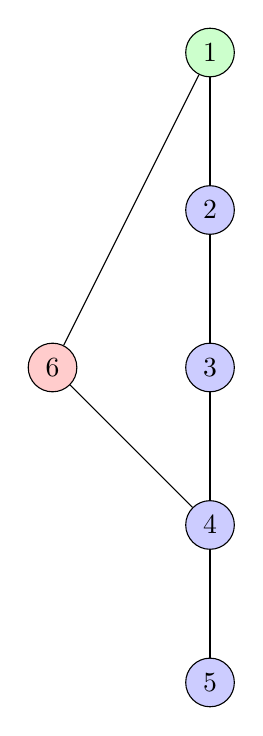
\begin{tikzpicture}
		[
			p1/.style={circle, draw, fill=green!20},
			p2/.style={circle, draw, fill=blue!20},
			p3/.style={circle, draw, fill=red!20},
		]

		% Nodes
		\foreach \style/\name/\x/\y in
		{
			p1/1/2/8,
			p2/2/2/6,
			p2/3/2/4,
			p2/4/2/2,
			p2/5/2/0,
			p3/6/0/4
		}
			\node[\style] (\name) at (\x,\y) {\name};

		% Edges
		\foreach \u/\v in
		{
			1/2,
			1/6,
			2/3,
			3/4,
			4/5,
			6/4}
			\draw (\u) -- (\v);

		\end{tikzpicture}
	}
	\caption{\label{subfig:graph}}
	\end{subfigure}
	~
	% Single Source Query Coordinator Model
	\begin{subfigure}{0.2\textwidth}
	\scalebox{0.7}{
		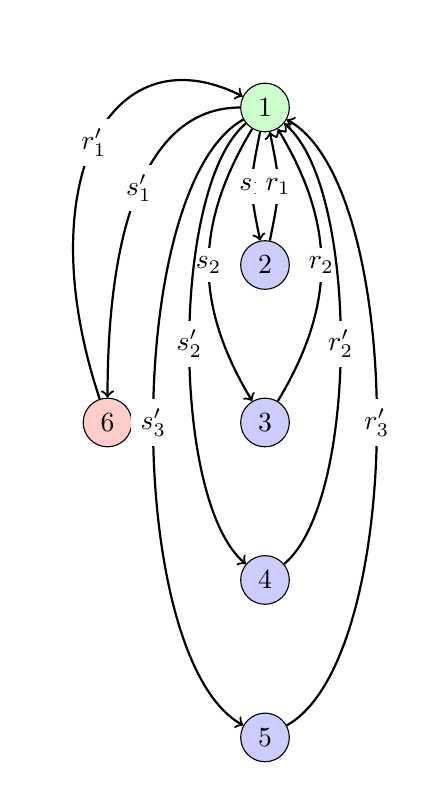
\begin{tikzpicture}
		[
			p1/.style={circle, draw, fill=green!20},
			p2/.style={circle, draw, fill=blue!20},
			p3/.style={circle, draw, fill=red!20},
		]

		% Nodes
		\foreach \style/\name/\x/\y in
		{
			p1/1/2/8,
			p2/2/2/6,
			p2/3/2/4,
			p2/4/2/2,
			p2/5/2/0,
			p3/6/0/4
		}
			\node[\style] (\name) at (\x,\y) {\name};

		% Requests
		\foreach \u/\v/\a/\b/\text in
		{
			1/2/{( 1.8,  7  )}/{( 1.8,  7  )}/$s_1 $,
			2/1/{( 2.2,  7  )}/{( 2.2,  7  )}/$r_1 $,
			1/6/{( 0.5,  8  )}/{( 0  ,  6.5)}/$s_1'$,
			6/1/{(-1  ,  7  )}/{( 0  ,  9  )}/$r_1'$,
			1/3/{( 1.1,  6.5)}/{( 1.1,  5.5)}/$s_2 $,
			3/1/{( 2.9,  5.5)}/{( 2.9,  6.5)}/$r_2 $,
			1/4/{( 0.8,  7  )}/{( 0.8,  3  )}/$s_2'$,
			4/1/{( 3.2,  3  )}/{( 3.2,  7  )}/$r_2'$,
			1/5/{( 0.2,  7  )}/{( 0.2,  1  )}/$s_3'$,
			5/1/{( 3.8,  1  )}/{( 3.8,  7  )}/$r_3'$
		}
			\draw[thick, ->] (\u) .. controls \a and \b .. node[fill=white] {\text} (\v);

		\end{tikzpicture}
	}
	\caption{\label{subfig:sscquery}}
	\end{subfigure}
	~
	% State Passing Query Coordinator Model
	\begin{subfigure}{0.2\textwidth}
	\scalebox{0.7}{
		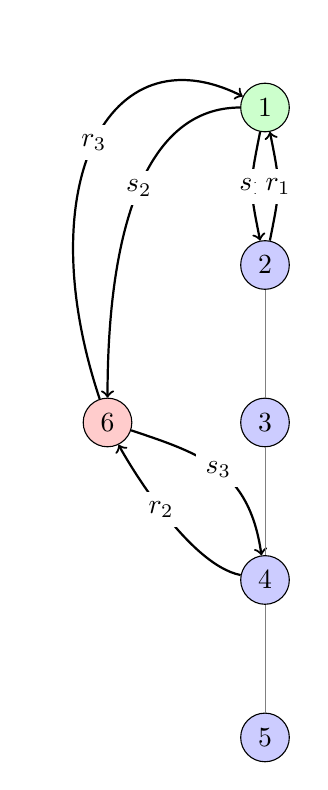
\begin{tikzpicture}
		[
			p1/.style={circle, draw, fill=green!20},
			p2/.style={circle, draw, fill=blue!20},
			p3/.style={circle, draw, fill=red!20},
		]

		% Nodes
		\foreach \style/\name/\x/\y in
		{
			p1/1/2/8,
			p2/2/2/6,
			p2/3/2/4,
			p2/4/2/2,
			p2/5/2/0,
			p3/6/0/4
		}
			\node[\style] (\name) at (\x,\y) {\name};

		% Requests
		\foreach \u/\v/\a/\b/\text in
		{
			1/2/{( 1.8,  7  )}/{( 1.8,  7  )}/$s_1$,
			2/1/{( 2.2,  7  )}/{( 2.2,  7  )}/$r_1$,
			1/6/{( 0.5,  8  )}/{( 0  ,  6.5)}/$s_2$,
			6/1/{(-1  ,  7  )}/{( 0  ,  9  )}/$r_3$,
			6/4/{( 1.2,  3.6)}/{( 1.8,  3.4)}/$s_3$,
			4/6/{( 1  ,  2.2)}/{( 0.2,  3.6)}/$r_2$
		}
			\draw[thick, ->] (\u) .. controls \a and \b .. node[fill=white] {\text} (\v);

		% Edges
		\foreach \u/\v in
		{
			2/3,
			3/4,
			4/5}
			\draw[help lines] (\u) -- (\v);

		\end{tikzpicture}
	}
	\caption{\label{subfig:spcquery}}
	\end{subfigure}
	~
	% Distributed State and Query Coordinators Model
	\begin{subfigure}{0.2\textwidth}
	\scalebox{0.7}{
		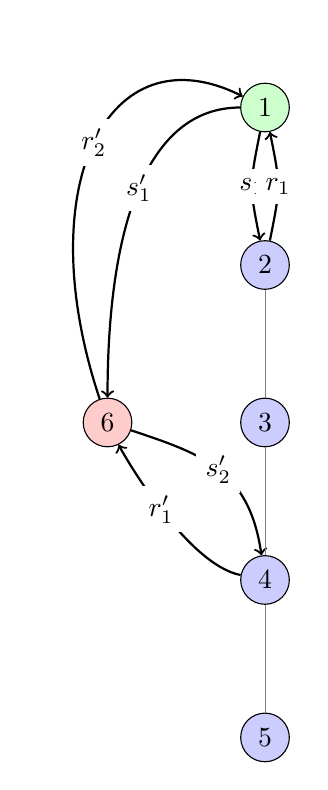
\begin{tikzpicture}
		[
			p1/.style={circle, draw, fill=green!20},
			p2/.style={circle, draw, fill=blue!20},
			p3/.style={circle, draw, fill=red!20},
		]

		% Nodes
		\foreach \style/\name/\x/\y in
		{
			p1/1/2/8,
			p2/2/2/6,
			p2/3/2/4,
			p2/4/2/2,
			p2/5/2/0,
			p3/6/0/4
		}
			\node[\style] (\name) at (\x,\y) {\name};

		% Requests
		\foreach \u/\v/\a/\b/\text in
		{
			1/2/{( 1.8,  7  )}/{( 1.8,  7  )}/$s_1 $,
			2/1/{( 2.2,  7  )}/{( 2.2,  7  )}/$r_1 $,
			1/6/{( 0.5,  8  )}/{( 0  ,  6.5)}/$s_1'$,
			6/1/{(-1  ,  7  )}/{( 0  ,  9  )}/$r_2'$,
			6/4/{( 1.2,  3.6)}/{( 1.8,  3.4)}/$s_2'$,
			4/6/{( 1  ,  2.2)}/{( 0.2,  3.6)}/$r_1'$
		}
			\draw[thick, ->] (\u) .. controls \a and \b .. node[fill=white] {\text} (\v);

		% Edges
		\foreach \u/\v in
		{
			2/3,
			3/4,
			4/5}
			\draw[help lines] (\u) -- (\v);

		\end{tikzpicture}
	}
	\caption{\label{subfig:dscquery}}
	\end{subfigure}
\caption{\ref{subfig:graph}: A graph with 3 partitions. We show the execution of
a 3-hop Neighborhood Search in the 3 query models presented in
Section~\ref{sec:distributedqueryproc}, starting at vertex $1$.
\ref{subfig:sscquery}: Getting a remote vertex always requires a network call.
\ref{subfig:spcquery}: State is passed to the partition where the query would
normally flow. Each partition is visited in sequence.  \ref{subfig:dscquery}:
State is maintained in a distributed manner. Control can flow in parallel to
each partition.}
\label{fig:querymodels}
\end{figure*}

\subsubsection{Single Source Query Coordinator}
\label{sec:singlesourcequerycoord}

This model is agnostic of partitioning. Queries are executed at the starting
partition as if all vertices are local. When a remote vertex is required because
of some edge traversal, it is retrieved from the remote partition with a network
call. The advantage of this model is that it abstracts query execution from data
layout, so that query state is maintained at a single source, that can always
coordinate traversals in an optimal way.

An example of this execution can be seen in Figure~\ref{subfig:sscquery}, when
answering the 3NR query starting at vertex $1$. Since each vertex is remote,
they are brought over the network in iterative fashion. Vertices $\{2, 6\}$ can
be brought in parallel, with separate requests $s_1$ and $s_1'$.

The disadvantage of this model is the amount of network requests that need
to be made -- 5 in Figure~\ref{subfig:sscquery}. Even for vertices such as
$\{4,5\}$ that are located on the same partition and traversed together, we
require sending two network requests to retrieve them. This inability of
accessing nodes that are co-located also hurts in terms of caching. A remote
partition that is accessed by a query, and stores intermediate results for that
query in its cache, cannot use those results.

\subsubsection{State Passing Query Coordinator}
\label{sec:statepassingquerycoord}

This model passes the current state of a query to the remote partition required
to be visited next because of an inter-partition edge. This is used to reduce
the amount of network calls required for traversing edges. For example in
Figure~\ref{subfig:spcquery}, while satisfying the 3NR query, and traversing the
edge $(1, 2)$, we pass all the current visited vertices, as the state of the
query, to the blue partition. There, the edges $(2, 3)$ and $(3, 4)$ are
traversed locally, and state is returned to the green partition, which continues
its execution.

The disadvantage of this model is that, although the number of network messages
decreases, the amount of data sent per network message increases -- sometimes
considerably depending on the graph layout. Furthermore, queries are no longer
independent of the partitioning of data. For example, in
Figure~\ref{subfig:spcquery}, vertex $4$ is visited twice as part of the 3NR
query. Once when traversing edge $(3, 4)$, when it is at a distance of 3-hops
from $1$, and once when traversing edge $(6, 4)$, when it is at a distance of
2-hops from $1$. As such, queries like 3NR which are breadth-first search in
nature, need to be modified to fit the iterative deepening style of traversal.
Lastly, this model requires sequential execution, despite the fact that multiple
edges can be traversed in parallel in the original query, as seen in
Section~\ref{sec:singlesourcequerycoord}. This is due to the fact that state
passes along the edges.

\subsubsection{Distributed State and Query Coordinators}
\label{sec:distributedstatequerycoord}

This model maintains a distributed state of the query at the partitions that are
accessed. This is achieved by generating unique query IDs, which are passed to
remote partitions together with the continuation of the query. Each partition
tags the vertices that are visited by a query with the query ID and the
appropriate state determined by the query continuation.

For example, in Figure~\ref{subfig:dscquery}, while executing the 3NR query,
when edge $(1, 6)$ is traversed, the query ID, the number of remaining
hops (2) and the current hop count (1) is passed to the red partition. This is
used to tag vertex $6$ as being at distance $1$ within the specified query, and
a continuation follows while traversing edge $(6, 4)$.

The benefit of this model is that minimal information needs to be passed during
network calls -- the query ID and state that is constant in size. This is in
contrast to the previous model, where state was proportional to the query result
size. Furthermore, in this model, edges can be traversed in parallel, as state
is maintained in a distributed manner by each partition. In the provided
example, edges $(1, 2)$ and $(1, 6)$ can be traversed in parallel.

The disadvantage of this approach is that a vertex such as $4$ can be visited
twice, with different distance metrics, depending on the ordering of the
parallel requests. Thus, like in the previous mode, a query needs to be modified
since it is no longer independent of the partitioning and traversal schema.
